\documentclass[11pt]{article}
\usepackage[a4paper,margin=0.8in]{geometry}
\usepackage{amsmath,amssymb,amsthm,mathtools}
\usepackage{enumitem,microtype,graphicx}
\usepackage[dvipsnames]{xcolor}
\usepackage[colorlinks=true,linkcolor=MidnightBlue,citecolor=MidnightBlue,urlcolor=MidnightBlue]{hyperref}
\setlist{nosep,leftmargin=*}
\newtheorem{theorem}{Theorem}
\newtheorem{corollary}[theorem]{Corollary}
\newcommand{\Om}{\Omega}
\newcommand{\C}{\mathbb C}
\newcommand{\K}{\mathcal K}
\title{The canonical bundle map of an essential $C([0,1])$-module\\
\large A counterexample to the injectivity question in arXiv:1005.4561}
\author{Autonomous solve-first investigation, lane 12}
\date{12 August 2026}

\begin{document}
\maketitle

\begin{abstract}
Leung, Ng, and Wong ask whether the canonical map from every essential Banach
$C(\Omega)$-module to its associated section module is injective when
$\Omega$ is a compact subset of $\mathbb R$.  The answer is no, already for
$\Omega=[0,1]$.  With its usual multiplication action,
$F=L^1([0,1])$ is an essential Banach $C([0,1])$-module, but every canonical
fiber $F/K_\omega^F$ is zero.  Consequently the canonical map is identically
zero.  The same phenomenon occurs for every $L^p$-module over an atomless
finite regular measure, $1\le p<\infty$.
\end{abstract}

\section{The question}

Let $F$ be an essential Banach $C(\Om)$-module.  For $\omega\in\Om$, the
source defines
\[
 K_\omega=\{a\in C(\Om):a(\omega)=0\},\qquad
 K_\omega^F=\overline{F K_\omega},
\]
and the canonical fiber $\Xi_\omega^F=F/K_\omega^F$.  The canonical map is
\begin{equation}\label{eq:canonical}
 \iota_F:F\longrightarrow\Gamma_0(\Xi^F),\qquad
 \iota_F(x)(\omega)=x+K_\omega^F.
\end{equation}
The closure of its image is denoted by $\widetilde F$.

Remark 4.10(b) of the source asks whether \eqref{eq:canonical} is injective
for every compact $\Om\subseteq\mathbb R$ and every essential Banach
$C(\Om)$-module $F$ \cite[p.~13]{LNW}.  Figure~\ref{fig:source} reproduces
the exact passage.

\begin{figure}[ht]
  \centering
  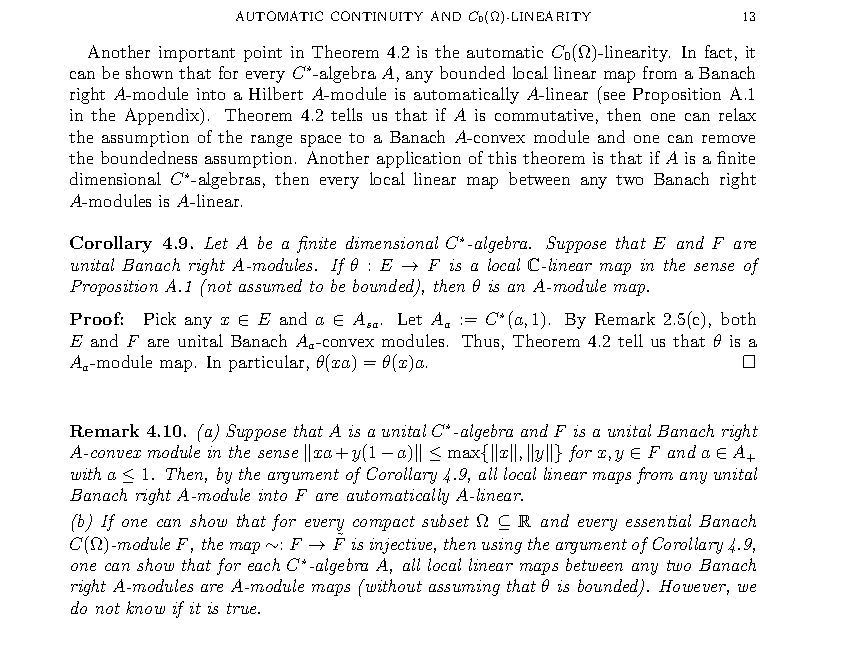
\includegraphics[width=0.72\linewidth]{figures/source_open_question.png}
  \caption{The injectivity question in Remark 4.10(b) of
  arXiv:1005.4561, p.~13.}
  \label{fig:source}
\end{figure}

\section{A maximally noninjective example}

\begin{theorem}\label{thm:main}
Let $\Om=[0,1]$, let $F=L^1([0,1])$ with respect to Lebesgue measure, and
give $F$ the right $C([0,1])$-module action
\[
                         x\cdot a=xa.
\]
Then $F$ is an essential Banach $C([0,1])$-module and
\[
                         K_\omega^F=F
                         \qquad(\omega\in[0,1]).       \tag{2}
\]
Hence every fiber $\Xi_\omega^F$ is zero, $\widetilde F=\{0\}$, and the
canonical map $\iota_F$ is the zero map.  In particular, it is not injective.
\end{theorem}

\begin{proof}
The action is bounded because
\[
                       \|xa\|_1\le \|x\|_1\|a\|_\infty.
\]
It is unital, so the Banach module is essential.

Fix $\omega\in[0,1]$.  For $m\ge1$, define
\[
                 a_m(t)=\min\{1,m|t-\omega|\},
                 \qquad 0\le t\le1.
\]
Then $a_m\in C([0,1])$, $a_m(\omega)=0$, and $0\le a_m\le1$.  Thus
$a_m\in K_\omega$.  Moreover, $a_m(t)\to1$ at every
$t\ne\omega$.  For arbitrary $x\in L^1([0,1])$,
\[
 |x(t)a_m(t)-x(t)|\le |x(t)|.
\]
Also, $x(t)a_m(t)\longrightarrow x(t)$ for almost every $t$.
Dominated convergence gives $\|xa_m-x\|_1\to0$.  Each $xa_m$ belongs to
$F K_\omega$, so $x\in\overline{F K_\omega}=K_\omega^F$.  Since $x$ was
arbitrary, $K_\omega^F=F$.

The argument holds for every $\omega$.  Therefore all quotients
$F/K_\omega^F$ vanish and \eqref{eq:canonical} sends every element to the
zero section.  As $L^1([0,1])\ne\{0\}$, the map is not injective.
\end{proof}

\begin{corollary}[atomless $L^p$ family]\label{cor:lp}
Let $\Om$ be a compact Hausdorff space carrying a nonzero finite regular
atomless Borel measure $\mu$.  For every $1\le p<\infty$, the canonical map
for the essential module $L^p(\Om,\mu)$ is identically zero.
\end{corollary}

\begin{proof}
For fixed $\omega$, regularity and $\mu(\{\omega\})=0$ give a decreasing net
of neighborhoods $U$ with $\mu(U)\to0$.  By normality of compact Hausdorff
spaces, choose $a_U\in C(\Om)$ such that $0\le a_U\le1$,
$a_U(\omega)=0$, and $a_U=1$ off $U$.  Then for $x\in L^p$,
\[
 \|x-xa_U\|_p^p\le\int_U |x|^p\,d\mu\longrightarrow0.
\]
Thus $K_\omega^{L^p}=L^p$ for every $\omega$, exactly as above.
\end{proof}
\paragraph{Scope.}
Theorem~\ref{thm:main} answers the stated injectivity question negatively,
and in the strongest possible way: the associated section representation can
lose the entire module.  Remark 4.10(b) presents injectivity as a sufficient
route to proving that arbitrary local maps between Banach right
$C^*$-modules are module maps.  The present counterexample blocks that route;
it does not by itself decide the broader local-map assertion.

{\small
\begin{thebibliography}{9}
\bibitem{LNW}
C.-W. Leung, C.-K. Ng, and N.-C. Wong,
\emph{Automatic continuity and $C_0(\Omega)$-linearity of linear maps between
$C_0(\Omega)$-modules}, J. Operator Theory 67 (2012), 3--24;
arXiv:1005.4561.
\end{thebibliography}
}

\end{document}
